%! Author = amatarazzo
%! Date = 06/04/24

\chapter{Foundations of Large Language Models}
\label{ch:foundations-of-large-language-models}

Large Language Models (LLMs) have revolutionized the field of Natural Language Processing (NLP) by achieving state-of-the-art performance on a wide range of tasks, such as text generation, text classification, and machine translation.\\
These models are trained on vast amounts of text data to learn the underlying structure of the language and capture the relationships between words.\\

In the following sections, we will explore the key concepts and techniques that underpin the development of LLMs, including pre-training strategies and major datasets used for training and evaluation, as well as the Transformer architecture, which forms the basis of many modern LLMs.\\

Finally, we will discuss some model adaptation techniques that can be used to fine-tune LLMs for specific tasks or domains.

\section{Pre-training}
\label{sec:pre-training}

Pre-training constitutes a foundational phase in the development of Large Language Models (LLMs).
It allows the model to capture the relationships between words and generate coherent and contextually relevant text, laying the groundwork for its subsequent performance on specific NLP tasks~\cite{devlin2019bert, brown2020language}.\\
This phase involves training a language model on a vast corpus of text data before fine-tuning it on a smaller, task-specific dataset, such as text generation or text classification, to improve its performance on that task.\\
Moreover, the extensive pre-training on diverse corpora enables LLMs to develop a broad understanding, making them adaptable to a wide range of domains and languages~\cite{liu2019roberta, radford2019language}.\\
Despite its advantages, pre-training LLMs is not without its challenges.
The process requires substantial computational resources and energy, raising concerns about its environmental impact~\cite{strubell2019energy}.
Additionally, the data used for pre-training can influence the model's biases and sensitivities, necessitating careful curation of the training corpus to mitigate potential ethical and fairness issues~\cite{bender2021dangers}.

The field is evolving towards more efficient pre-training methods, such as transfer learning, where a pre-trained model is adapted to new tasks or languages with minimal additional training~\cite{ruder2019transfer}.
Moreover, emerging approaches aim to enhance the contextual awareness and ethical sensitivity of LLMs during the pre-training phase, addressing the challenges of bias and fairness head-on.\\

\subsection{Pre-training strategies}
\label{subsec:pre-training-strategies}

There are several pre-training strategies that have been used to train large language models, including unsupervised pre-training, supervised pre-training, and semi-supervised pre-training.
Let's explore each of these strategies in more detail.

\subsubsection{Unsupervised pre-training}
\label{subsubsec:unsupervised-pre-training}

Unsupervised pre-training is a pre-training strategy that involves training a model on a large corpus of text data without any labels or annotations.\\
The model is trained to predict the next word in a sequence of words, given the previous words in the sequence~\cite{brown2020language}.
This is done using a technique called Autoregressive Language Modeling (ALM), where the model is trained to predict the probability distribution over the next word in the sequence given the previous words in the sequence in a unidirectional manner.\\
Models like GPT-3 and its variants use this autoregressive language modeling objective to pre-train on large text corpora and learn the relationships between words in the language.\\
The main idea behind ALM is the prediction of the next token in a sequence based on the tokens that precede it.
The computational realization of this modeling approach is typically achieved through neural networks, particularly transformers, which leverage self-attention mechanisms to encapsulate dependencies across varying distances in the input sequence~\cite{vaswani2023attention}.

During the generation process, a token is sampled based on the probability distribution predicted by the model for the next token position, appended to the sequence, and this augmented sequence is then fed back into the model iteratively to generate subsequent tokens~\cite{brown2020language}.
Despite its prowess, the autoregressive nature of these models imbues them with an intrinsic limitation: the inability to leverage future context in token prediction, constraining their context comprehension to a unidirectional scope.\\
BERT and its variants, on the other hand, employ a masked language model (MLM) objective, where random words in a sentence are masked, and the model is trained to predict these masked words based on their context, integrating both preceding and succeeding context in representation learning~\cite{devlin2019bert}.


\subsubsection{Supervised pre-training}
\label{subsubsec:supervised-pre-training}

Supervised pre-training is a pre-training strategy that involves training a model on a large corpus of text data with labels or annotations.
This paradigm contrasts with unsupervised pre-training, where models learn from raw text without explicit labels.
The supervised approach enables models to learn representations that are more closely aligned with the end tasks, potentially enhancing their performance and efficiency~\cite{gururangan2020don}.

\begin{figure}[h]
	\centering
	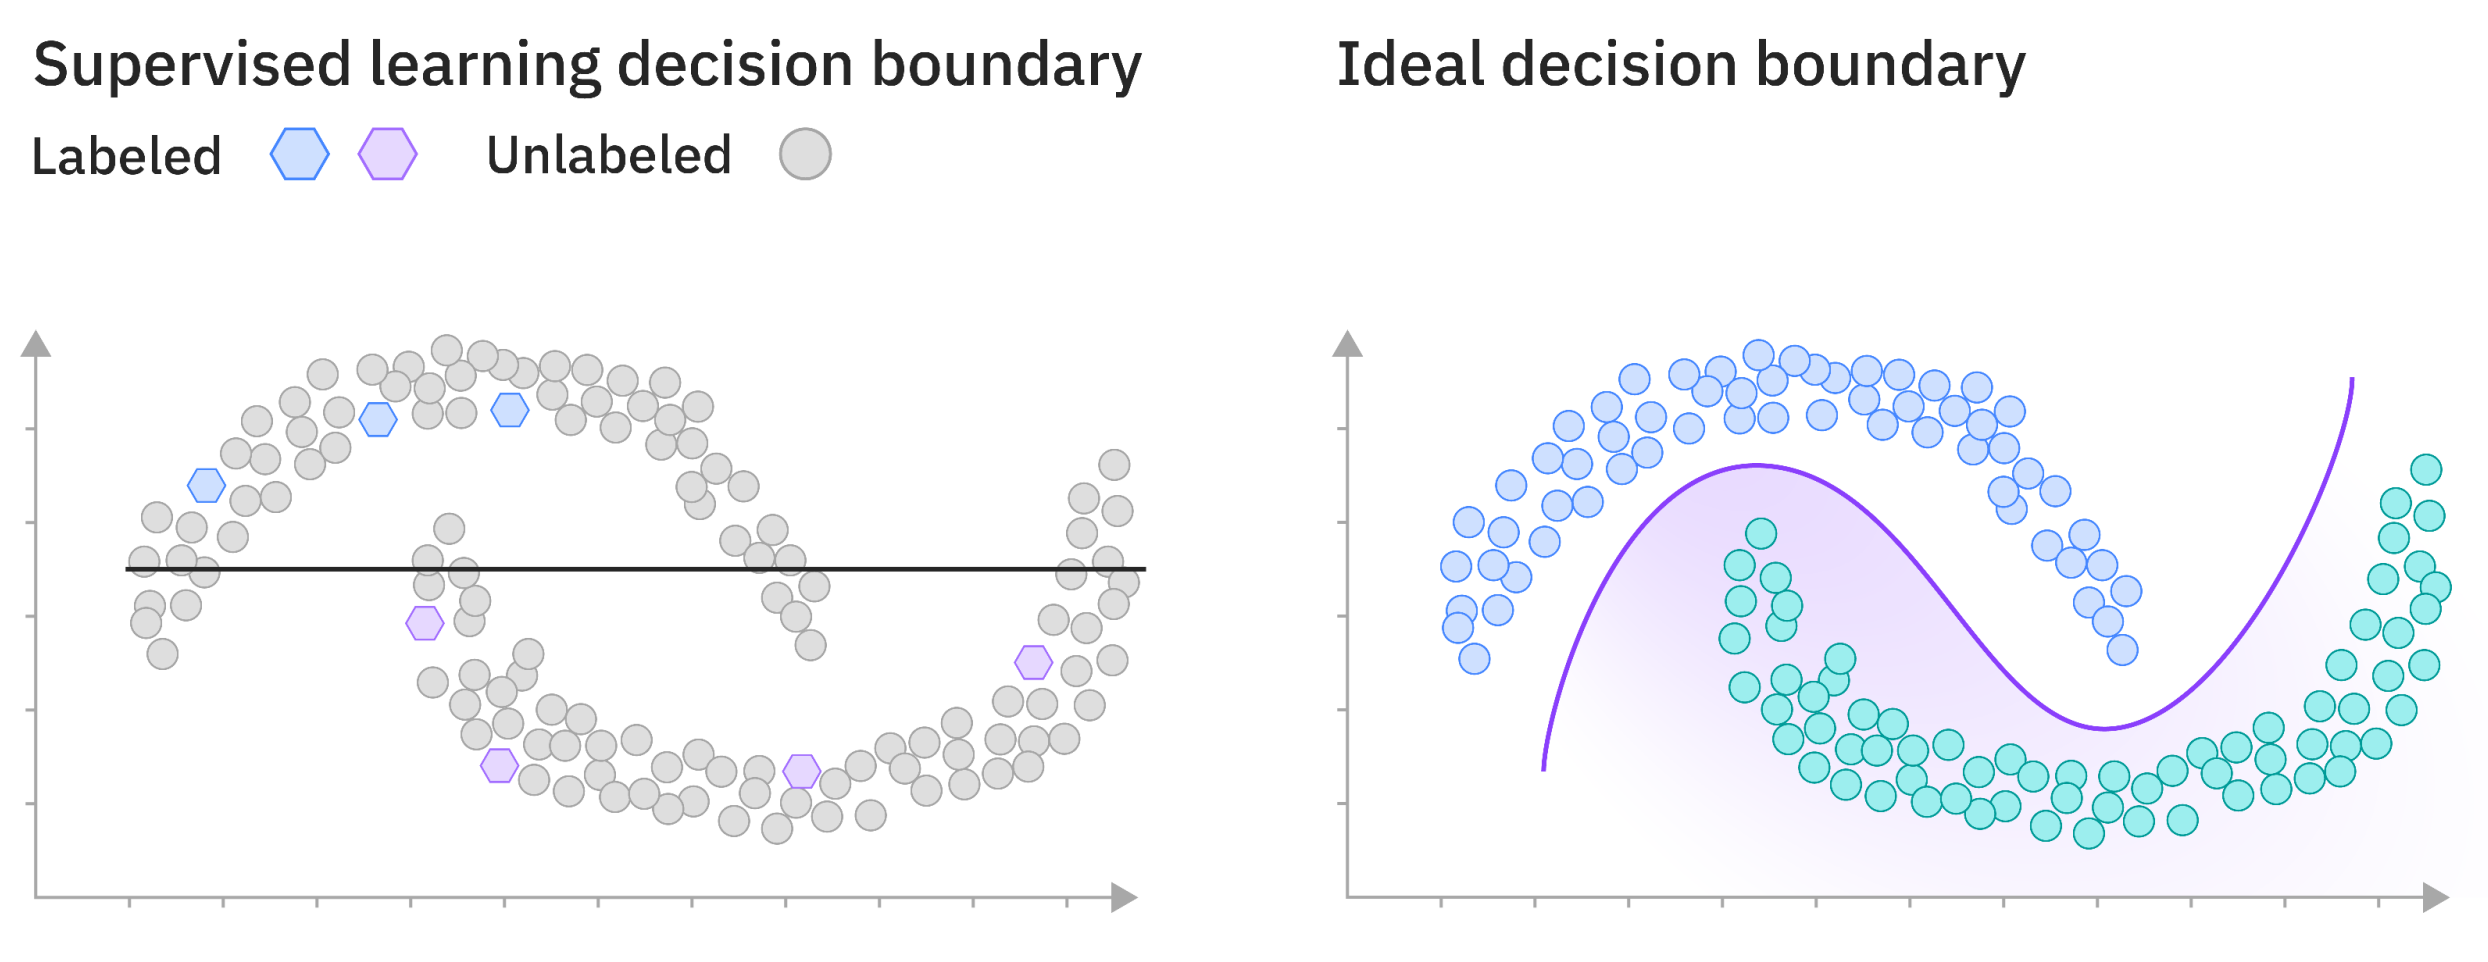
\includegraphics[width=\textwidth]{supervised}
	\caption{Using only the very limited labeled data points available, a supervised model may learn a decision boundary that will generalize poorly and be prone to misclassifying new examples. Source: \textcite{bergmann2023semi}.}
	\label{fig:supervised}
\end{figure}

In supervised pre-training, LLMs are exposed to a vast array of labeled data across various domains.
This training regime involves teaching the model to predict the correct output given an input, under the supervision of known input-output pairs.
This approach not only helps in learning general language representations but also imbues the model with domain-specific knowledge, which is particularly beneficial when the subsequent fine-tuning task is closely related to the pre-training data~\cite{phang2019sentence}.

One significant advantage of supervised pre-training is its potential to reduce the amount of labeled data required for fine-tuning on specific tasks.
By learning robust representations during pre-training, LLMs can achieve high performance on downstream tasks even with relatively smaller datasets, a concept known as transfer learning~\cite{ruder2019transfer}.
Moreover, supervised pre-training can lead to improvements in model generalization, making LLMs more adept at handling unseen data or tasks that diverge from their initial training corpus.\\

The reliance on large labeled datasets introduces concerns regarding the cost and feasibility of data annotation, especially in specialized domains where expert knowledge is required.\\
Furthermore, as shown in Figure~\ref{fig:supervised}, the risk of overfitting to the pre-training data is non-trivial, necessitating careful regularization and validation to ensure the model's generalizability~\cite{howard2018universal}.

\subsubsection{Semi-supervised pre-training}
\label{subsubsec:semi-supervised-pre-training}

Semi-supervised pre-training emerges as a compelling paradigm in the evolution of Large Language Models (LLMs), blending the strengths of supervised and unsupervised learning methodologies.
This hybrid training approach leverages a combination of labeled and unlabeled data, optimizing the utilization of available information and enhancing the model's learning efficacy and adaptability~\cite{zhu2005semi, chapelle2009semi}.

At its core, semi-supervised pre-training involves the initial training of models using a vast corpus of unlabeled data, akin to unsupervised pre-training.
This phase allows the model to capture a broad understanding of language structures and patterns.
Subsequently, the model undergoes further training or fine-tuning on a smaller labeled dataset, which instills task-specific knowledge and nuances~\cite{ruder2019transfer, yang2017transfer}.
The rationale behind this approach is to exploit the abundance of readily available unlabeled data to develop a comprehensive language model, which is then refined using the more scarce labeled data to achieve superior performance on target tasks.
Various techniques underpin semi-supervised pre-training in LLMs.

One prominent method involves self-training, where the model, initially trained on labeled data, generates pseudo-labels for the unlabeled dataset.
These pseudo-labeled data points are then incorporated into further training cycles, iteratively enhancing the model's accuracy and robustness~\cite{lee2013pseudo}.

Another notable technique is the use of consistency regularization, which ensures that the model produces similar outputs for perturbed versions of the same input data, enhancing the model's stability and generalization capabilities~\cite{sajjadi2016regularization}.

Other key techniques in semi-supervised learning include transductive and inductive learning, with practical methods like label propagation and active learning aiding in leveraging unlabeled data.
These approaches are instrumental in refining the model's decision-making capabilities~\cite{bergmann2023semi}.\\
Transductive learning, a concept primarily attributed to \textcite{vapnik1998statistical}, focuses on predicting specific examples from the training set without attempting to generalize beyond those.
In transductive inference, the model is directly applied to the specific test set, aiming to infer the correct labels for the given unlabeled data.

The key characteristic distinguishing transductive learning from other machine learning methods is its focus on the particular sample at hand rather than on a general rule applicable to new, unseen instances.\\
One of the main applications of transductive learning is in the realm of support vector machines (SVMs), where it is employed to predict labels for a given, fixed set of test data, optimizing the margin not only for the training data but also for the test data, despite their labels being unknown~\cite{joachims1999transductive}.

Conversely, inductive learning aims to build a general model that predicts outcomes for new, unseen data based on the patterns learned from the training data.
Label propagation (Figure~\ref{fig:label_propagation}) is a common technique in inductive learning, where the model infers the labels of unlabeled data points based on the labels of their neighbors in the feature space.

\begin{figure}[h]
	\centering
	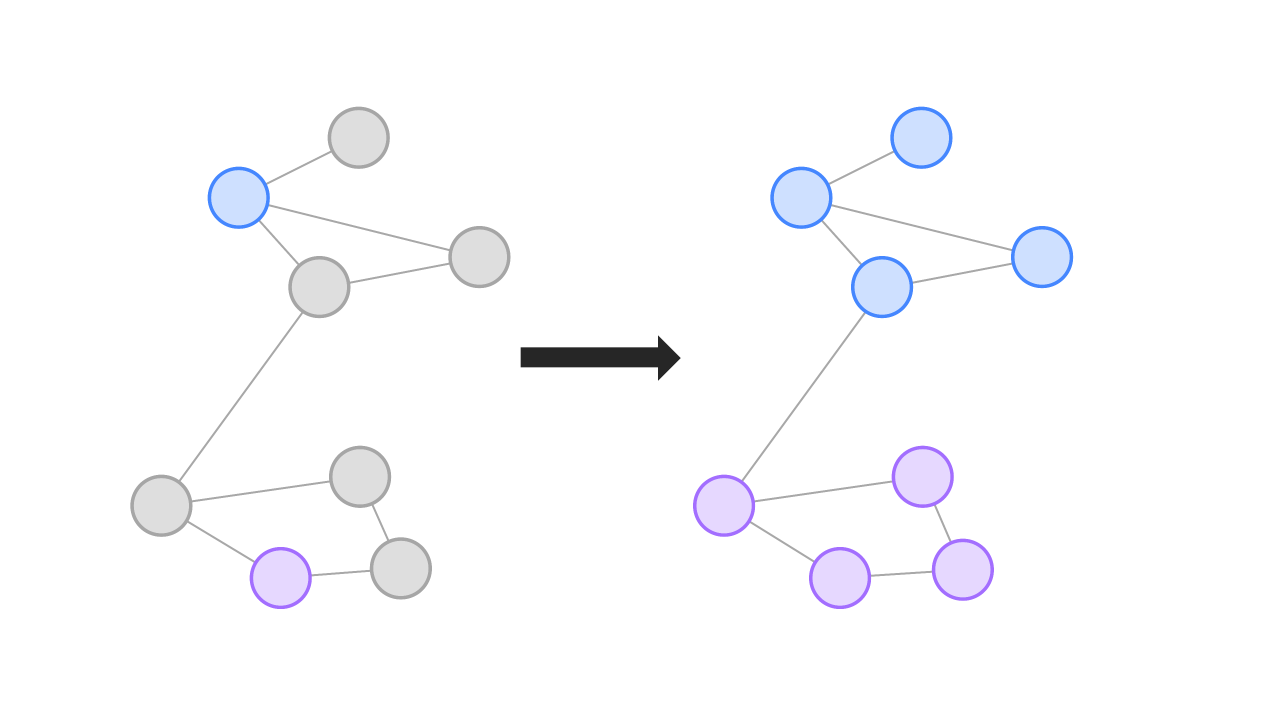
\includegraphics[width=\textwidth]{label_propagation}
	\caption{LEFT: original labeled and unlabeled data points. RIGHT: using label propagation, the unlabeled data points have been assigned pseudo-labels. Source: \textcite{bergmann2023semi}.}
	\label{fig:label_propagation}
\end{figure}

Active learning is another inductive learning method that involves iteratively selecting the most informative data points for labeling, optimizing the model's performance with minimal labeled data.
This approach is more general than transductive learning and underpins most supervised learning algorithms.
The objective here is to infer a function that can generalize well across unseen samples, not just the examples provided during the training phase.
Inductive learning is fundamental to numerous machine learning algorithms, from linear regression to deep neural networks, where the model learns an underlying function that maps input data to output predictions, with the hope that this function will perform accurately on data not present in the training set~\cite{mitchell1997machine}.

Semi-supervised approach is predicated on certain assumptions about the underlying structure and distribution of the data, which facilitate the effective integration of unlabeled data into the learning process.
\begin{itemize}
	\item \textbf{Cluster Assumption:} {The cluster assumption posits that data points within the same cluster are more likely to share a label. This assumption underpins the idea that data points in high-density regions of the input space belong to the same class, while low-density regions denote boundaries between classes~\cite{chapelle2009semi}. This principle guides the model to generalize from labeled data points to nearby unlabeled ones within the same cluster.}
	\item \textbf{Continuity Assumption:} {Also known as the smoothness assumption, this posits that if two points in the input space are close to each other, than their corresponding outputs are also likely to be similar~\cite{zhou2004learning}. In practical terms, this means that if two data points are close in the feature space, they are likely to share the same label.}
	\item \textbf{Manifold Assumption:} {The manifold assumption suggests that high-dimensional data lie on a low-dimensional manifold. This assumption implies that the data points are situated on a manifold of much lower dimensionality embedded within the higher-dimensional space, and learning can be simplified if this manifold structure is discovered and exploited~\cite{belkin2006manifold}. The manifold assumption often complements the cluster and continuity assumptions, providing a geometric interpretation of the data's distribution.}
	\item \textbf{Low-Density Separation Assumption:} {This assumption posits that the decision boundary between different classes should lie in regions of low data density~\cite{chapelle2009semi}. Essentially, it is expected that there is a natural separation or gap between classes, and the learning algorithm should prefer hypotheses that place the decision boundary in regions where few data points are present.}
\end{itemize}

\subsection{Data source}
\label{subsec:data-source}

Large Language Models (LLMs) exhibit a strong dependency on extensive, high-caliber data for pre-training, with their efficacy closely tied to the nature and preprocessing of the utilized corpora.
The main sources of data for training and evaluating LLMs can be broadly categorized into general and specialized datasets, each serving distinct purposes in enhancing the models' capabilities~\cite{survey}.\\

\begin{figure}[h]
	\centering
	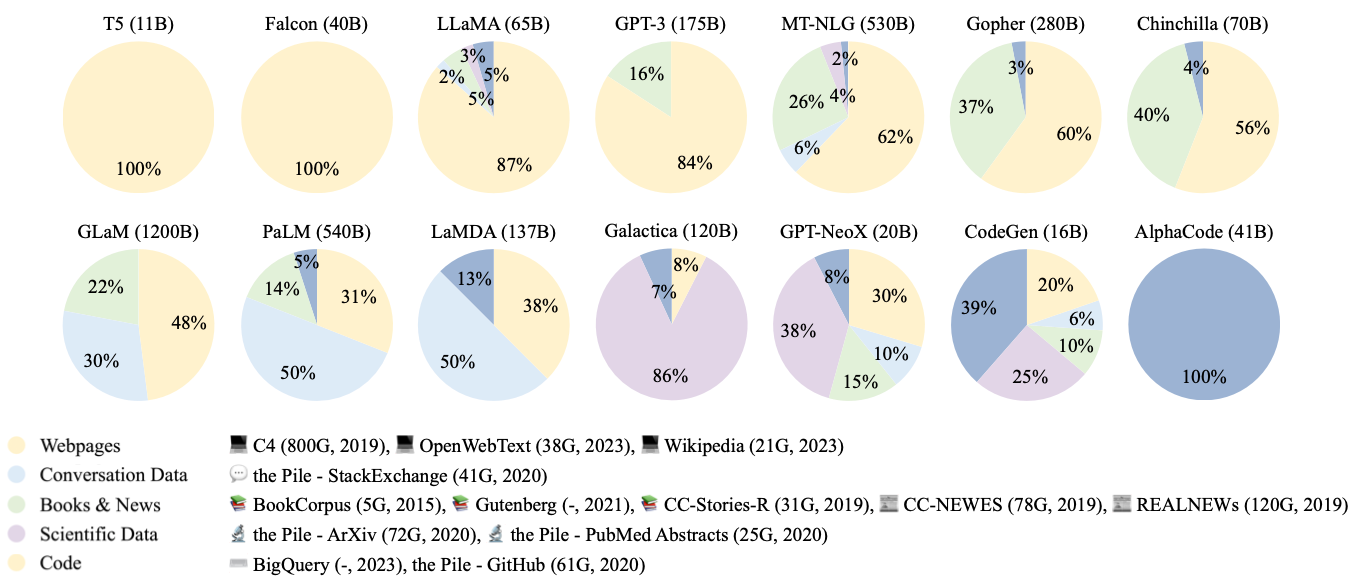
\includegraphics[width=\textwidth]{datasources}
	\caption{Commonly-used data sources for training and evaluating Large Language Models (LLMs). Source: \textcite{survey}.}
	\label{fig:data_sources}
\end{figure}

\textbf{General Data:} This category typically encompasses web content, literary works, and conversational texts, prized for their voluminous, varied, and accessible nature, thereby bolstering the language modeling and generalization prowess of LLMs. The inclusion of general data, such as web pages and books, offers a rich lexicon spanning various themes, essential for the comprehensive training of LLMs. As shown in Figure~\ref{fig:data_sources}, general purpose data are among the most commonly used general data sources for training LLMs.\\
Three important general data sources are:
\begin{itemize}
	\item \textbf{Webpages:} {Web content, extracted from the internet, is a valuable source of diverse and up-to-date text data, encompassing news articles, blog posts, and forum discussions. This data is instrumental in training LLMs to gain different linguistic knowledge and enhance generalization capabilities~\cite{brown2020language, raffel2023exploring}.
		      Crawled web data tend be a mix of high-quality and noisy text, necessitating careful preprocessing to ensure the data's quality and relevance.
	      }
	\item \textbf{Conversation text:} {
		      Conversation text, including chat logs and social media interactions, provides a rich source of informal language and colloquial expressions, enabling LLMs to capture the nuances of human communication~\cite{zhang2022opt}. This data is particularly useful for training LLMs on question answering~\cite{chowdhery2022palm} and sentiment analysis tasks~\cite{zellers2019defending}.\\
		      Conversational data often involve multiple speakers, so an effective way is to trasform the conversation in a tree structure, where the utterance is linked to the one it is replying to. The tree can be divided in multiple subtrees, each one representing a sub-conversation, which can be collected in the pre-training corpus.
		      Overtraining on conversational data can lead to the model to a performance decline, since the declarative instructions and direct interrogatives can be erroneously interpreted as the beginning of a conversation~\cite{zhang2022opt}.
	      }
	\item \textbf{Books:} {
		      Books, comprising novels, essays, and scientific literature, offer a rich source of long structured and coherent text data, enabling LLMs to learn complex language structures and thematic nuances~\cite{zhu2015aligning}. This data is instrumental in training LLMs on literary text generation tasks and enhancing their proficiency in narrative comprehension and storytelling~\cite{radford2019language}.
	      }
\end{itemize}

\textbf{Specialized Data:} Tailored to refine LLMs' proficiency in particular tasks, specialized datasets encompass multilingual text, scientific literature, and programming code.
Specialized datasets are useful to improve the specific capabilities of LLMs on downstream tasks.
Next, we introduce three kinds of specialized data.
\begin{itemize}
	\item \textbf{Multilingual text:} {
		      Multilingual text data, spanning multiple languages and dialects, is crucial for training LLMs to understand and generate text in diverse linguistic contexts~\cite{survey}. This data is instrumental in enhancing the models' cross-lingual capabilities and enabling them to perform translation tasks across different languages~\cite{survey}.
		      BLOOM~\cite{workshop2023bloom} and PaLM~\cite{chowdhery2022palm} are two models that have been trained on multilingual text data to improve their performance on cross-lingual tasks. They have impressive performances on translation, multilingual question answering, and cross-lingual summarization tasks, and they achieve comparable or superior results to models fine-tuned on specific languages.
	      }
	\item \textbf{Scientific literature:} {
		      Scientific literature, encompassing research papers, patents, and technical documents, provides a rich source of domain-specific text data, essential for training LLMs on scientific text generation and reasoning tasks~\cite{survey, taylor2022galactica, lewkowycz2022minerva}.
		      To build the scientific corpus for training LLMs, existing efforts mainly collect arXiv papers, scientific textbooks, math web-pages, and other related scientific resources.
		      Data in sceintific fields are complex, commonly including mathematical symbols and protein sequences, so specific tokenization and preprocessing techniques are required to transform these different formats of data into a unified form that can be processed by language models.
	      }
	\item \textbf{Code:} {
		      Code, encompassing source code snippets and software documentation, is a valuable source of structured text data, essential for training LLMs on code generation and code completion tasks~\cite{survey, nijkamp2022codegen}.
		      Code data is often collected from open-source repositories like GitHub and StackOverflow, and it is used to train LLMs to generate code snippets, complete code fragments, and perform code summarization tasks.
		      Recently ~\textcite{chen2021evaluating, austin2021program} have shown that models trained on code data can be used to generate code with high accuracy and efficiency, and they can be used to improve the performance of code completion tasks. Generated code can successfully pass expert-designed unit-test cases~\cite{chen2021evaluating} or solve competitive programming problems~\cite{li2022competition}.
		      In general, two types of code corpora are used: one is question answering datasets like Stack Exchange~\cite{xu2022systematic}; the second is public software repositoris like GitHub~\cite{chen2021evaluating} where code, comments and docstring are collected for utilization.
	      }
\end{itemize}

\subsubsection{Commonly-used data sources}
\label{subsec:commonly-used-data-sources}

The development and evaluation of Large Language Models (LLMs) rely heavily on the availability of high-quality datasets that span diverse domains and languages.
The datasets in Table~\ref{tab:table} serve as the foundation for pre-training and fine-tuning LLMs, enabling researchers to assess the models' performance on a wide range of tasks, from text generation to translation.\\

\begin{table}[h]
	\centering
	\begin{tabularx}{\textwidth}{|X|X|X|X|}
		\hline
		\textbf{Corpora}                           & \textbf{Size} & \textbf{Source} & \textbf{Update Time} \\
		\hline
		BookCorpus~\cite{zhu2015aligning}          & 5GB           & Books           & Dec-2015             \\
		Gutenberg~\cite{projectgutenberg}          & -             & Books           & Dec-2021             \\
		C4~\cite{raffel2023exploring}              & 800GB         & CommonCrawl     & Apr-2019             \\
		CC-Stories-R~\cite{trinh2018simple}        & 31GB          & CommonCrawl     & Sep-2019             \\
		CC-NEWS~\cite{liu2019roberta}              & 78GB          & CommonCrawl     & Feb-2019             \\
		REALNEWS~\cite{zellers2019defending}       & 120GB         & CommonCrawl     & Apr-2019             \\
		OpenWebText~\cite{gokaslan2019openwebtext} & 38GB          & Reddit links    & Mar-2023             \\
		Pushift.io~\cite{baumgartner2020pushshift} & 2TB           & Reddit links    & Mar-2023             \\
		Wikipedia~\cite{wikipedia}                 & 21GB          & Wikipedia       & Mar-2023             \\
		BigQuery~\cite{bigquerydataset}            & -             & Codes           & Dec-2023             \\
		the Pile~\cite{gao2021pile}                & 800GB         & Other           & Dec-2020             \\
		ROOTS~\cite{laurencon2022bigscience}       & 1.6TB         & Other           & Jun-2022             \\
		\hline
	\end{tabularx}
	\caption{Statistics of commonly-used data sources. Source: \textcite{survey}}
	\label{tab:table}
\end{table}

In this section, we will explore some of the most commonly-used data sources for training and evaluating LLMs.
Based on their content types, we categorize these corpora into six groups: Books, CommonCrawl, Reddit links, Wikipedia, Code, and others.

\begin{itemize}
	\item \textbf{Books:} {
		      BookCorpus~\cite{zhu2015aligning} and Gutenberg~\cite{projectgutenberg} are two prominent datasets that contain text from a wide range of books, spanning various genres and topics. These datasets are valuable for training LLMs on literary text and assessing their performance on text generation tasks.\\
		      BookCorpus is a dataset consisting of text from over 11,000 books (e.g., novels and biographies), while Gutenberg is a collection of over 70,000 free ebooks including novels, essays, poetry, drama, history, science, philosophy, and other types of works in the public domain.\\
		      BookCorpus is commonly used in previous small-scale models (e.g., GPT~\cite{radford2018improving} and GPT-2~\cite{radford2019language}), while Gutenberg is used in more recent large-scale models (i.e., LLaMa~\cite{touvron2023llama}).\\
		      Book1 and Book2 used in GPT-3~\cite{brown2020language} are much larger than BookCorpus, but they have not been publicly released.
	      }
	\item \textbf{CommonCrawl:} {
		      CommonCrawl~\cite{commoncrawl} is a vast web corpus that contains data from billions of web pages, covering diverse topics and languages. Due to noise and redundancy in the data, researchers often extract subsets of CommonCrawl for training LLMs. The main subsets used for training LLMs are C4\footnote{Colossal Clean Crawled Corpus}~\cite{raffel2023exploring}, CC-Stories-R~\cite{trinh2018simple}, CC-NEWS~\cite{liu2019roberta}, and REALNEWS~\cite{zellers2019defending}.\\
	      }
	\item \textbf{Reddit links:} {
		      Reddit is a social media platform where users can submit links and posts and "upvotes" or "downvote" them. Posts with high number of "upvotes" are often considered useful, and can be used to create high-quality datasets.
		      OpenWebText~\cite{gokaslan2019openwebtext} and Pushshift.io~\cite{baumgartner2020pushshift} are datasets that contain text data extracted from Reddit. These datasets are useful for training LLMs on social media text and assessing their performance on text generation and sentiment analysis tasks.
	      }
	\item \textbf{Wikipedia:} {
		      Wikipedia~\cite{wikipedia} is a widely-used dataset that contains text from articles on various topics. It's an online encyclopedia with a large volume of high-quality articles. Most of these articles are composed in an expository style of writing (with supporting references), covering a wide range of languages and fields.
		      Typically, the English-only filtered versions of Wikipedia are widely used in most LLMs (e.g., GPT-3~\cite{brown2020language}, and LLaMA~\cite{touvron2023llama}).
		      Wikipedia is available in multiple languages, so it can be used in multilingual settings.
	      }
	\item \textbf{Code:} {
		      Two major sources are GitHub, for open-source licensed code, and StackOverflow, for code-related question-answering platforms.\\
		      Google has publicly released BigQuery~\cite{bigquerydataset}, a dataset that contains code snippets from various programming languages. This dataset is useful for training LLMs (i.e., CodeGen~\cite{nijkamp2022codegen}) on code text and assessing their performance on code generation and code completion tasks.
	      }
	\item \textbf{Others:} {
		      The Pile~\cite{gao2021pile} and ROOTS~\cite{laurencon2022bigscience} are datasets that contain text data from various sources, such as books, articles, and websites.\\
		      The Pile contains 800GB of data from multiple sources, including books, websites, codes, scientific papers, and social media platforms. It's widely used in training LLMs with different size (e.g., CodeGen(16B)~\cite{nijkamp2022codegen} and Megatron-Turing NLG(530B)~\cite{smith2022deepspeed}).\\
		      ROOTS is composed of various smaller datasets (totally 1.61 TB of text) in 59 different languages (containing natural languages and programming languages). It's been used for training BLOOM~\cite{workshop2023bloom}.
	      }
\end{itemize}

In practice, a mixture of these datasets is often used to train LLMs, as they provide a diverse range of text data (Figure~\ref{fig:data_sources}).
The choice of datasets depends on the specific task and domain of interest, as well as the computational resources available for training the model.
Furthermore, to train LLMs that are adaptative to specific tasks or domains, is also important to consider the data sources that are relevant to them.\\

\subsection{Data preprocessing}
\label{subsec:data-preprocessing}

After collecting the data, the next step is to preprocess it to ensure that it is clean, consistent, and ready for training Large Language Models (LLMs) removing noise and irrelevant, or potentially toxic information~\cite{chowdhery2022palm, rae2021scaling, longpre2023pretrainer}.
In \textcite{chen2023datajuicer} the authors propose a new data preprocessing system, DataJuicer, that can be used to improve quality of the processed data.\\
A typical pipeline for data preprocessing involves several steps, as shown in Figure~\ref{fig:preprocessing}:

\begin{figure}[H]
	\centering
	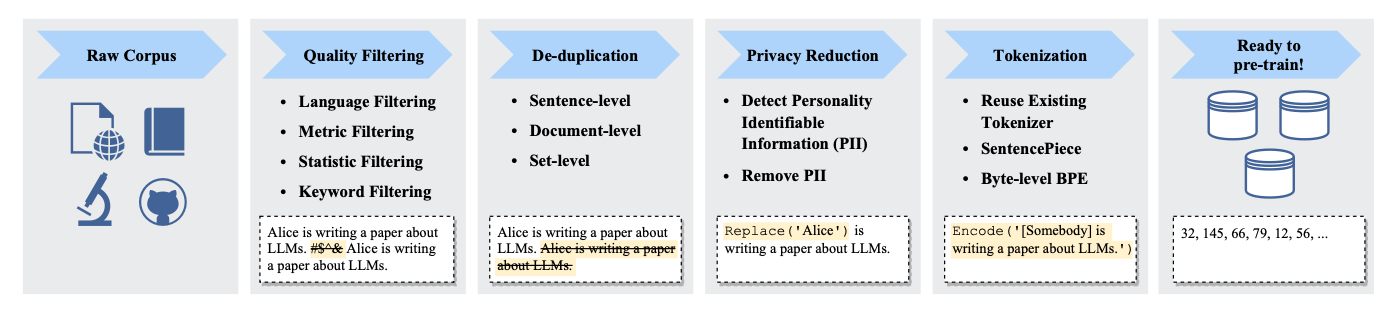
\includegraphics[width=\textwidth]{preprocessing}
	\caption{Common data preprocessing steps for training Large Language Models (LLMs). Source: \textcite{survey}.}
	\label{fig:preprocessing}
\end{figure}

\textbf{Quality Filtering.}
The first step in data preprocessing is quality filtering, where the data is cleaned to remove irrelevant or low-quality content.
Existing works mainly adopt two strategies for quality filtering: classifier-based and heuristic-based filtering.
The former approach involves training a classifier to distinguish between high-quality and low-quality data, using well-curated data (e.g., Wikipedia pages) as positive examples and noisy data (e.g., spam or irrelevant content) as negative examples.
\textcite{rae2021scaling, du2022glam} find that classifier-based filtering may remove high-quality data in dialect, colloquial, and sociolectal\footnote{In sociolinguistics, a sociolect is a form of language or a set of lexical items used by a socioeconomic class, profession, age group, or other social group. Sociolects involve both passive acquisition of particular communicative practices through association with a local community, as well as active learning and choice among speech or writing forms to demonstrate identification with particular groups. Source: \textcite{wikipedia}} languages, which potentially leads to bias in the pre-training data and diminishes the corpus diversity.\\
Heuristic-based filtering, on the other hand, involves setting predefined rules to identify and remove noisy data~\cite{workshop2023bloom, rae2021scaling}.
The set of rules can be summarized as follows:
\begin{itemize}
	\item \textit{Language based filtering}: {Remove data that is not in the target language.}
	\item \textit{Metric based filtering}: {Remove data that does not meet certain quality metrics, e.g., perplexity, readability, or coherence.
	      Perplexity (PPL) is one of the most common metrics for evaluating language models.
	      This metric applies specifically to classical language models (sometimes called autoregressive or causal language models) and is not well-defined for masked language models like BERT~\cite{devlin2019bert}.
	      Perplexity is defined as the exponential average negative log-likelihood of a sequence.
	      If we have a tokenized sequence \(X = x_1, x_2, \ldots, x_t\), the perplexity of the sequence is defined as:
	      \begin{equation}
		      PPL(X) = \exp \left\{ -\frac{1}{t} \sum_{i}^{t} \log p_{\theta}(x_i | x_{<i}) \right\}
		      \label{eq:equation_perplexity}
	      \end{equation}
	      where \(\log p_{\theta}(x_i | x_{<i})\) is the log-likelihood of the token \(x_i\) given the previous tokens \(x_{<i}\) in the sequence.
	      Intuitively, it can be thought of as an evaluation of the model’s ability to predict uniformly among the set of specified tokens in a corpus\footnote{This means that the tokenization procedure has a direct impact on a model’s perplexity which should always be taken into consideration when comparing different models.}~\cite{huggingface2023perplexity}.
	      }
	\item \textit{Statistic based filtering}: {
	      statistical features like punctuation distribution, symbol-to-word ratio, and sentence length can be used to filter out low-quality data.
	      }
	\item \textit{Keyword based filtering}: {Remove data that contains specific keywords that are noisy, irrelevant or toxic like HTML tags, URLs, boilerplate text, or offensive language.}
\end{itemize}

\textbf{Deduplication.}
The next step in data preprocessing is deduplication, where duplicate data  are removed to reduce redundancy and improve the diversity of the training data.
Moreover, \textcite{hernandez2022scaling} found that duplication may cause instability in the training process, leading to overfitting and poor generalization performance.
Therefore, deduplication is essential to ensure that the model is exposed to a diverse range of text data during training.
It can be done at various granularity, such as at the document level, paragraph level, or sentence level.
Low-quality sentences that contains repeated words or phrases can be removed to improve the quality of the data.
At document level, the deduplication can be done by computing overlap ratio of surface features (e.g., words and n-grams overlap) between documents, and removing the duplicates that contains similar contents~\cite{touvron2023llama,rae2021scaling,workshop2023bloom,lee2022deduplicating}.
To avoid the contamination problem, the deduplication process should be done before the data is split into training, validation, and test sets~\cite{chowdhery2022palm}.
\textcite{chowdhery2022palm} and \textcite{carlini2022quantifying} have shown that the three deduplication strategies should be used in conjunction to improve the training of LLMs.

\textbf{Privacy reduction.}
Privacy reduction is another important step in data preprocessing, especially when dealing with sensitive or personal information.
Since data is often collected from web and contains user-generated content, the risk of privacy breaching is high~\cite{carlini2021extracting}.
This step involves anonymizing or obfuscating sensitive data to protect the privacy of individuals.
Common techniques for privacy reduction include masking personally identifiable information (PII), such as names, addresses, and phone numbers, and replacing them with generic placeholders or tokens~\cite{laurencon2022bigscience}.\\
Privacy attacks to LLMs can be attributed to presence of duplicated PII data in the pre-training, which can be used to extract the original PII data~\cite{lee2022deduplicating}.
Therefore, de-duplication can also reduce privacy risks to some extent.

\textbf{Tokenization.}
Tokenization is a crucial step in data preprocessing, where the text data is converted into tokens that can be processed by the model.
The choice of tokenization method can have a significant impact on the model's performance, as different tokenization strategies can affect the model's ability to capture the underlying structure of the language.
Common tokenization techniques include word-based tokenization, subword-based tokenization, and character-based tokenization.
Word-based tokenization splits the text into individual words, while subword-based tokenization breaks down the text into subword units, such as prefixes, suffixes, and roots.
Character-based tokenization, on the other hand, tokenizes the text into individual characters.
Word-based tokenization is the predominant method used in traditional NLP research~\cite{lafferty2001conditional}.
However, word-based tokenization can be problematic for languages with complex morphology or limited vocabulary, as it may result in a large vocabulary size and sparse data representation.
In some other languages, like Chinese, Japanese, and Korean, word-based tokenization is not suitable because these languages do not have explicit word boundaries\footnote{It means that it can yield different segmentation results for the same input.}.
Thus, several neural network-based models employed subword-based tokenization, such as Byte Pair Encoding (BPE)~\cite{sennrich2016neural}, Unigram~\cite{kudo2018sentencepiece}, and WordPiece~\cite{wu2016google}, to address these challenges.\\

Byte Pair Encoding (BPE) is a type of data compression technique that has been effectively adapted for natural language processing tasks, particularly in the domain of tokenization for large language models (LLMs).
The BPE algorithm operates by iteratively merging the most frequent pair of bytes (or characters in the context of text) in a given dataset into a single, new byte (or character), and it repeats this process until a specified number of merges has been reached or another stopping criterion has been met.
The application of BPE in the field of NLP was popularized by \textcite{sennrich2016neural} in the context of neural machine translation.
They demonstrated that using BPE allowed for efficient handling of rare and unknown words, which are commonplace in languages with rich morphology or in specialized vocabularies, such as scientific texts or code.
By splitting words into subword units, BPE provides a balance between the granularity of characters and the semantic units of full words, enabling models to represent a wide vocabulary with a limited set of tokens.
BPE has been fundamental in the architecture of influential language models, such as OpenAI's GPT series, BART and LLaMA\@.\\

WordPiece tokenization is a tokenization method that segments text into subword units, allowing for a balance between the flexibility of character-based models and the efficiency of word-based models.
Originating from speech processing~\cite{wu2016google}, this method has found significant application in natural language processing, particularly within neural network-based models such as BERT and its variants.\\
In WordPiece tokenization, a base vocabulary is first constructed with individual characters, and then more frequent and meaningful sub-word units are incrementally added.
This construction process is guided by a criterion that aims to maximize the language model likelihood on a training corpus, thus ensuring that the resulting tokens are optimal representations for the given data.
The WordPiece algorithm iteratively merges the most frequently co-occurring pairs of tokens to form new sub-word units until a specified vocabulary size is reached.\\
This tokenization strategy has shown effectiveness in reducing out-of-vocabulary issues, as the model can fall back on smaller sub-word units when encountering unfamiliar words.
Moreover, by capturing sub-word regularities, WordPiece facilitates the learning of meaningful representations for morphologically rich languages within large language models.
This is particularly advantageous for handling agglutinative languages, where words often comprise a series of affixed morphemes\footnote{
	Agglutinative languages are a type of morphological linguistic classification in which words are formed through the linear addition of discrete units, each of which carries a specific grammatical meaning. These discrete units are known as morphemes, which are the smallest grammatical units in a language. In agglutinative languages, morphemes are concatenated in a way that each morpheme represents a single grammatical function, such as tense, number, case, or aspect.
	For example, in Turkish -- an agglutinative language -- a single word can be made up of a base or root word with several affixes attached to it to modify its meaning. These affixes remain relatively invariant; they don’t undergo significant changes in form when they’re combined with other morphemes. Here’s an illustrative example from Turkish:\\
	"ev" means "house"\\
	"evler" means "houses" (plural)\\
	"evlerim" means "my houses" (possessive plural)\\
	Each suffix attached to "ev" is a separate morpheme that changes the meaning of the word, indicating plurality and possession without ambiguity.
	This is in contrast to fusional languages, where a single affix can represent multiple grammatical categories, or isolating languages, where words generally do not change form at all, and grammatical relations are indicated by word order or separate words.
}.

Unigram tokenization is a statistical method that employs an unigram language model for the probabilistic segmentation of text into tokens.
This technique, standing in contrast to the deterministic nature of Byte Pair Encoding, involves constructing a unigram model from a large initial vocabulary and iteratively refining it to maximize the likelihood of the observed corpus~\cite{kudo2018sentencepiece}.
The essence of Unigram tokenization lies in its iterative pruning process, wherein less probable tokens are systematically eliminated from the vocabulary.
To estimate the unigram language model, it adopts an expectation–maximization (EM) algorithm: at each iteration, we first find the currently optimal tokenization of words based on the old language model, and then re-estimate the probabilities of unigrams to update the language model.
During this procedure, dynamic programming algorithms (i.e., the Viterbi algorithm) are used to efficiently find the optimal decomposition way of a word given the language model\cite{survey}.
This probabilistic approach is adept at handling the linguistic complexities and variations found across different languages and domains.
It particularly excels in the context of language models that require a nuanced understanding of morphological structures and sub-word variations.
Unigram tokenization has been pivotal in the development of the SentencePiece~\cite{kudo2018sentencepiece} tokenization library, which is renowned for its application in T5 and mBART.
The adaptability and language-agnostic properties of Unigram tokenization make it a preferred choice for LLMs tasked with processing multilingual data~\cite{kudo2018sentencepiece}.

\section{Architectures}
\label{sec:architectures}

The architecture of Large Language Models (LLMs) plays a pivotal role in determining the model's performance, efficiency, and scalability.

Generally speaking, we can identify some key components that define different LLM architectures: the encoder and the decoder.

The encoder is an essential component in LLMs, and its role is to process input sequences and map them to a higher dimensional space, capturing the contextual information in the data.
The structure of an encoder in LLMs typically involves a stack of identical layers, each comprising two main sub-layers: a multi-head self-attention mechanism and a position-wise fully connected feed-forward network~\cite{vaswani2023attention}.

The decoder, on the other hand, is responsible for generating output sequences based on the encoded representations.
The decoder in models such as GPT-3~\cite{brown2020language} and its successors operates on the principle of autoregressive modeling, where each subsequent token is predicted based on the previously generated tokens.
A key feature of decoders in LLMs is causality, which ensures that the prediction for the current token can only attend to previous tokens, not future ones.
This is implemented through masked attention mechanisms in the transformer's decoder layers~\cite{vaswani2023attention}.

For example, in a translation task, the encoder processes the source sentence and produces a set of vectors representing its content, while the decoder uses cross-attention to decide which words (or phrases) in the source sentence are most relevant for predicting the next word in the target language.
In code generation, decoders can create syntactically correct code snippets given comments or docstrings as input, as demonstrated by Codex~\cite{chen2021evaluating}.\\

Based on the components and the way they are connected, LLMs can be categorized into three main types: encoder-only\footnote{
	We refer to BERT-style methods as encoder-only, the description encoder-only may be misleading since these methods also decode the embeddings into output tokens or text during pretraining.
	In other words, both encoder-only and decoder-only architectures are "decoding". However, the encoder-only architectures, in contrast to decoder-only and encoder-decoder architectures, are not decoding in an autoregressive fashion.
	Autoregressive decoding refers to generating output sequences one token at a time, conditioning each token on the previously generated tokens.
	Encoder-only models do not generate coherent output sequences in this manner.
	Instead, they focus on understanding the input text and producing task-specific outputs, such as labels or token predictions~\cite{raschka2023encoderdecoder}.
},
decoder-only, and encoder-decoder models.
All of these methods are sequence-to-sequence models (often abbreviated as seq2seq).\\

\begin{figure}[H]
	\centering
	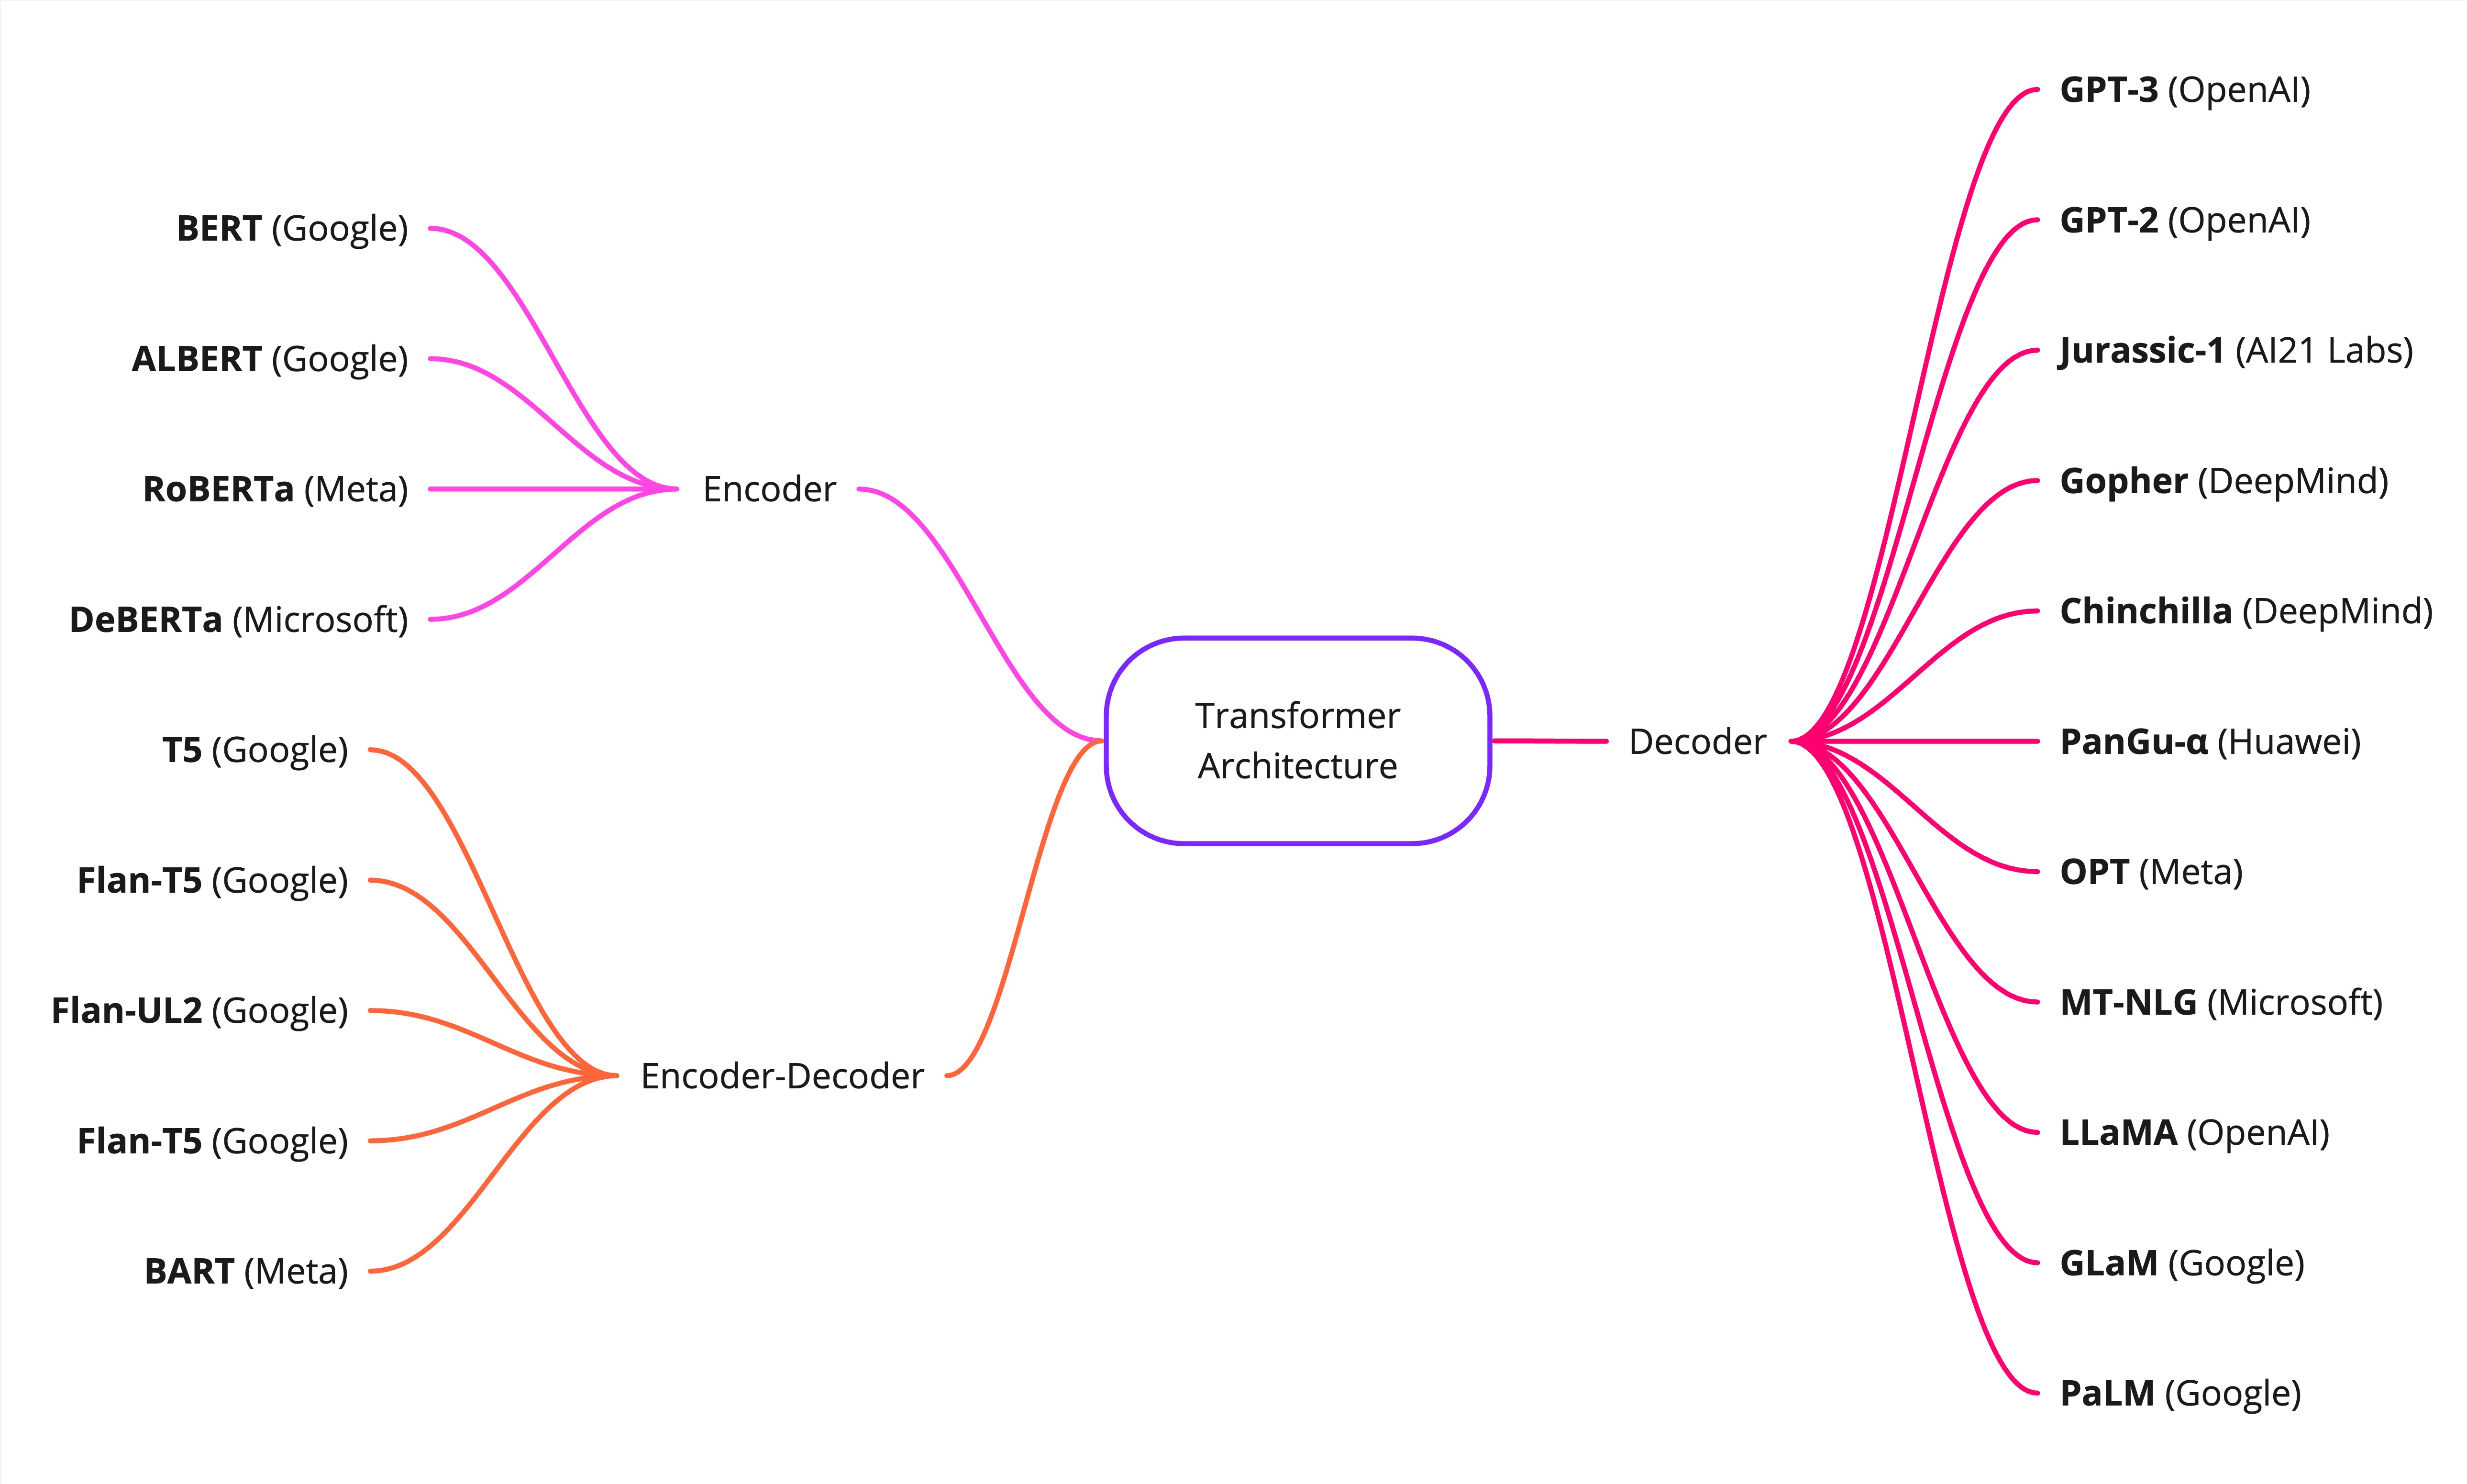
\includegraphics[width=\textwidth]{LLMs-Architectures}
	\caption{Some of the mainstream LLMs models by type.}
	\label{fig:llms-architectures}
\end{figure}

Mainstream architectures can be further categorized into three major types, namely encoder-decoder, casual decoder and prefix decoder as shown in Figure~\ref{fig:architectures}.
Both casual decoder and prefix decoder are decoder-only architectures, but they differ in the way they generate tokens.

\subsection{Encoder-decoder}
\label{subsec:encoder-decoder}

Vanilla version of the Transformer architecture introduced by \textcite{vaswani2023attention} belongs to this category, which consists of an encoder and a decoder.
The encoder's purpose is to transform an input sequence into a set of representations which capture its semantic and syntactic properties.
The decoder, on the other hand, is tasked with generating an output sequence from the encoded representations.
It predicts each token by conditioning on the previously generated tokens and the encoded input, a process that has seen significant improvements with the integration of cross-attention modules.
By segregating the understanding (encoding) and generation (decoding) processes, the Encoder-Decoder architecture enables a flexible approach to diverse language tasks.

So far, there are only a small number of models that use the encoder-decoder architecture (Figure~\ref{fig:llms-architectures}), such as BART~\cite{lewis2020bart} and T5~\cite{raffel2023exploring}.

\begin{figure}[h]
	\centering
	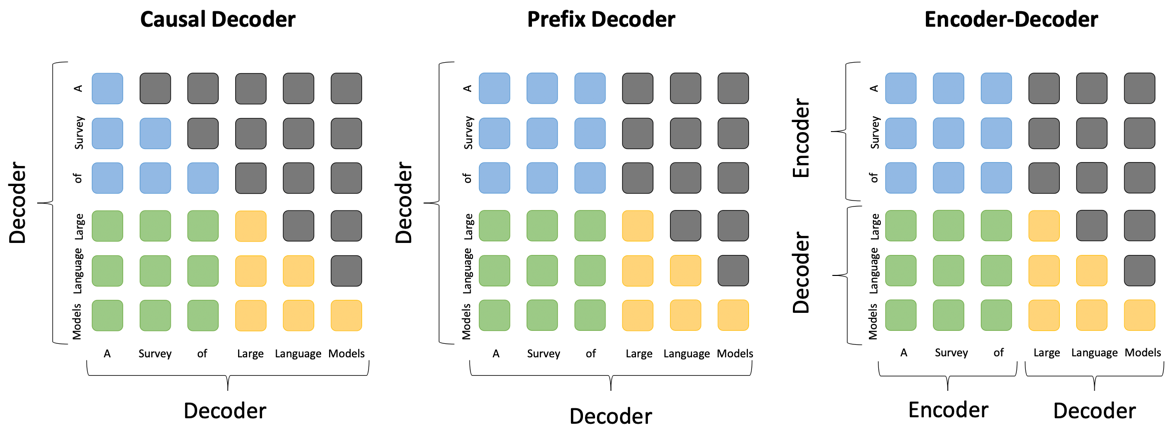
\includegraphics[width=\textwidth]{main_architectures}
	\caption{A comparison of the attention patterns in three mainstream architectures. Here, the blue, green, yellow and grey rounded rectangles indicate the attention between prefix tokens, attention between prefix and target tokens, attention between target tokens, and masked attention respectively. Source: \textcite{survey}.}
	\label{fig:architectures}
\end{figure}

\subsection{Casual decoder}
\label{subsec:casual-decoder}

In a causal decoder, each token is predicted based on the tokens that precede it, ensuring that the generation process is unidirectional and prevents the model from using future tokens in the prediction process~\cite{vaswani2023attention}.
This mechanism is akin to how humans produce language, one word at a time, building upon what has already been said without access to future words.

The architecture typically employs self-attention mechanisms where the attention distribution is masked to prevent tokens from attending to subsequent positions in the sequence (i.e., unidirectional attention mask).
This form of masking is instrumental in preserving the autoregressive property within the transformer-based models~
\cite{radford2019language}.

The GPT series\footnote{GPT-3~\cite{brown2020language} showed amazing in-context learning capability, whereas GPT-1~\cite{radford2018improving} and GPT-2~\cite{radford2019language} didn't. It seems that scaling plays an important role in increasing the model capacity of this model architecture} of language models by OpenAI are prominent examples that utilize causal decoder architectures, where the ability to generate coherent and contextually relevant text has been demonstrated effectively~\cite{brown2020language}.

The causal decoder architecture is particularly well-suited for tasks that require sequential generation, such as text completion, language modeling, and text generation.
It has been widely adopted as the architecture of choice for many large-scale language models, such as OPT~\cite{zhang2022opt}, BLOOM~\cite{workshop2023bloom}, and Gopher~\cite{rae2021scaling}.

\subsection{Prefix decoder}
\label{subsec:prefix-decoder}

The prefix decoder architecture\footnote{Also called non-causal decoder~\cite{zhang2022examining}} enables partial conditioning of generated sequences, revising the masking mechanism of causal decoders, to enable performing bidirectional attention over the prefix tokens~\cite{dong2019unified} and unidirectional attention only on generated tokens.
In other words, this architecture allows the model to generate tokens based on both the input prefix and the target prefix, which can be useful for tasks that require generating sequences with specific prefixes or constraints.
In practice, a prefix decoder is implemented by feeding a fixed sequence of tokens, known as the prefix, into the decoder alongside the tokens generated so far.
The model then extends the prefix by generating subsequent tokens that logically follow the context provided by the prefix.\\

Unlike the causal decoder, which strictly adheres to a unidirectional generation pattern, the prefix decoder allows for a predefined context or prefix to guide the generative process~\cite{li2021prefixtuning}.
This is particularly useful in tasks such as machine translation, where the prefix can be a part of the translation that is already known or hypothesized, but the flexibility provided by the prefix decoder makes it suitable for a range of applications, from controlled text generation to task-oriented dialog systems, where maintaining context and coherence is crucial~\cite{li2022ptuning}.

This architecture has been utilized in various language models to improve control over text generation and to enhance the models' ability to handle specific formats or styles~\cite{raffel2023exploring}.

\subsection{Transformer Architecture}
\label{subsec:transformer-architecture}

The Transformer architecture has emerged as the de facto standard for LLMs, owing to its ability to capture long-range dependencies and model complex language structures effectively~\cite{vaswani2023attention} making possible to train models with billions or even trillions of parameters~\cite{brown2020language, touvron2023llama}.
This architecture usually consists of stacked Transformer layers (Figure~\ref{fig:architecture}), each comprising multi-head self-attention sub-layer and a position-wise fully connected feed-forward network~\cite{vaswani2023attention}.
Residual connection~\cite{he2016deep} and layer normalization~\cite{ba2016layer} are applied for both sub-layers individually.

\begin{figure}[H]
	\centering
	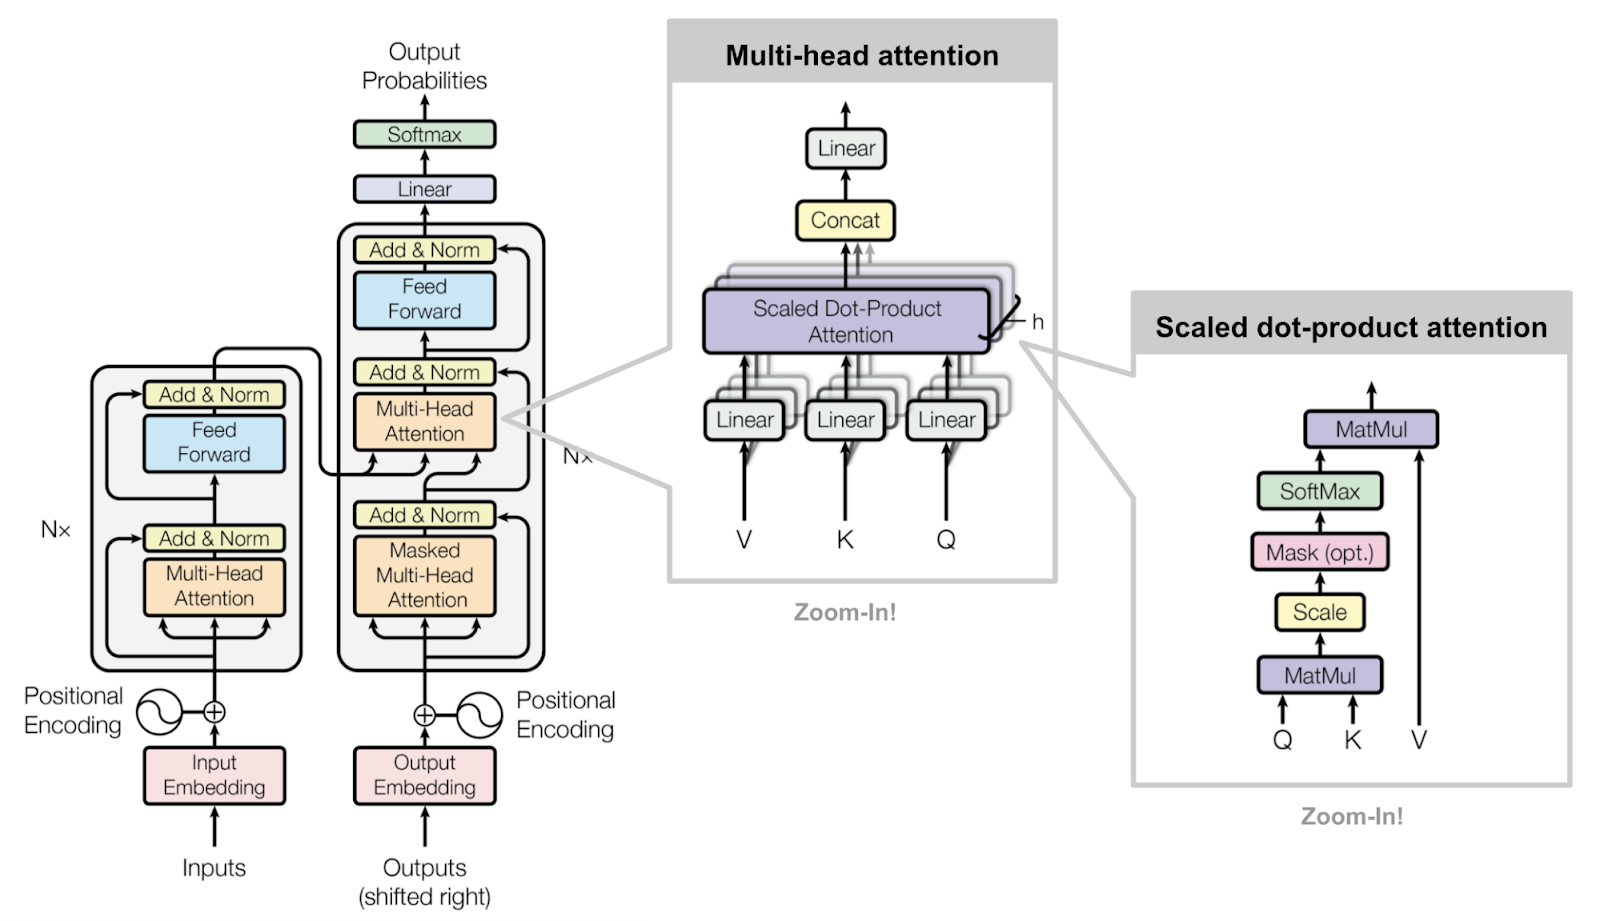
\includegraphics[width=0.6\textwidth]{transformer_architecture}
	\caption{The Transformer model architecture. Source: \textcite{vaswani2023attention}.}
	\label{fig:architecture}
\end{figure}

An attention function can be described as mapping a query and a set of key-value pairs to an output, where the query, keys, values, and output are all vectors.
The output is computed as a weighted sum of the values, where the weight assigned to each value is computed by a compatibility function of the query with the corresponding key.
The two most commonly used attention functions are additive attention~\cite{bahdanau2014neural}, and dot-product (multiplicative) attention.

\begin{figure}[h]
	\centering
	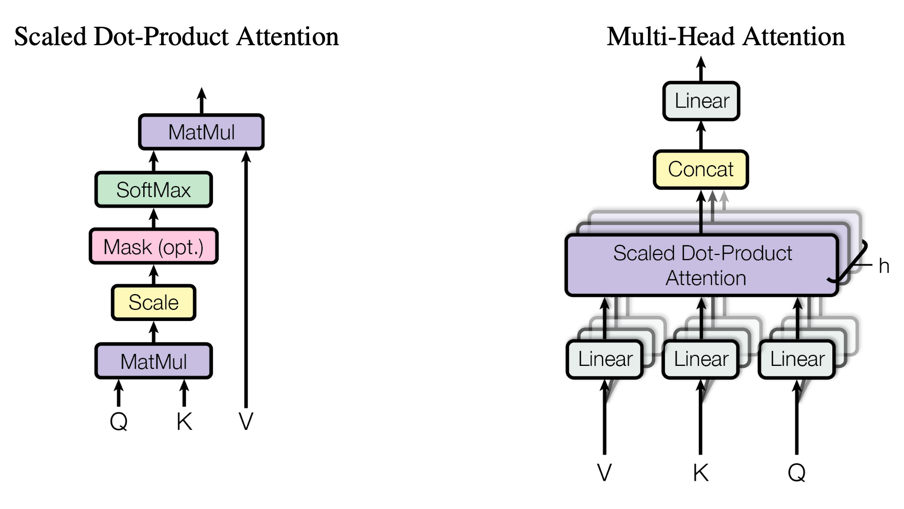
\includegraphics[width=0.8\textwidth]{attention}
	\caption{(left) Scaled Dot-Product Attention. (right) Multi-Head Attention consists of several attention layers running in parallel. Source: \textcite{vaswani2023attention}.}
	\label{fig:attention}
\end{figure}

The scaled dot-product attention function used in \textcite{vaswani2023attention} is defined as follows:

\begin{equation}
	\text{Attention}(Q, K, V) = \text{softmax}\left(\frac{QK^T}{\sqrt{d_k}}\right)V
	\label{eq:dot-scaled-attention}
\end{equation}

\noindent where \(Q\), \(K\), and \(V\) are the query, key, and value matrices, respectively, and d\textsubscript{k} is the dimension of the key vectors.
While for small values of d\textsubscript{k} the two mechanisms perform similarly, additive attention outperforms dot product attention without scaling for larger values of d\textsubscript{k}~\cite{britz2017massive}.
A multihead attention functions is implemented by splitting the query, key, and value vectors into multiple heads and computing the attention function in parallel, yielding d\textsubscript{v}-dimensional output values.
These are concatenated and once again projected, resulting in the final values, as depicted in Figure~\ref{fig:attention}.
The multihead attention mechanism allows the model to jointly attend to information from different representation subspaces at different positions, enhancing the model's capacity to capture complex relationships in the data.

\begin{equation}
	\begin{aligned}
		\text{MultiHead}(Q, K, V) & = \text{Concat}(\text{head}_1, \ldots, \text{head}_h)W^O, \\
		\text{head}_i             & = \text{Attention}(QW_i^Q, KW_i^K, VW_i^V)
	\end{aligned}
	\label{eq:multihead-attention}
\end{equation}

\noindent where \(W_i^Q\), \(W_i^K\), and \(W_i^V\) are the weight matrices for the query, key, and value projections of the \(i\)-th head, respectively, and \(W^O\) is the final output projection matrix.\\

The position-wise FFN sub-layer is a two-layer feed-forward network with a ReLU activation function between the layers.
Given a sequence of vectors \(h_1, h_2, \ldots, h_n\), the computation of a position-wise FFN sub-layer on any \(h_i\), as shown in Equation~\ref{eq:ffn}.

\begin{equation}
	\text{FFN}(h_i) = \text{ReLU}(h_{i}W^1 + b^1)W^2 + b^2
	\label{eq:ffn}
\end{equation}

\noindent where \(W^1\), \(W^2\), \(b^1\), and \(b^2\) are learnable parameters of the FFN sub-layer.

Besides the two sub-layers described above, the residual connection and layer normalization are also key components to the
Transformer.
Different orders and configuration of the sub-layers, residual connection and layer normalization in a Transformer layer lead to variants of Transformer architectures as shown in Table~\ref{tab:model-cards}.

\begin{table}[htb]
	\centering
	\scriptsize
	\begin{tabularx}{\textwidth}{|l|X|l|l|l|l|l|l|l|l|l|}
		\hline
		Model                                  & Category               & Size & Normalization & PE       & Activation & Bias & \#L & \#H & d\textsubscript{model} & MCL  \\
		\hline
		GPT3~\cite{brown2020language}          & Causal\newline decoder & 175B & Pre LayerNorm & Learned  & GeLU       & Y    & 96  & 96  & 12288                  & 2048 \\
		PanGU-\(\alpha\)~\cite{zeng2021pangu}  & Causal\newline decoder & 207B & Pre LayerNorm & Learned  & GeLU       & Y    & 64  & 128 & 16384                  & 1024 \\
		OPT~\cite{zhang2022opt}                & Causal\newline decoder & 175B & Pre LayerNorm & Learned  & ReLU       & Y    & 96  & 96  & 12288                  & 2048 \\
		PaLM~\cite{chowdhery2022palm}          & Causal\newline decoder & 540B & Pre LayerNorm & RoPE     & SwiGLU     & N    & 118 & 48  & 18432                  & 2048 \\
		BLOOM~\cite{workshop2023bloom}         & Causal\newline decoder & 176B & Pre LayerNorm & ALiBi    & GeLU       & Y    & 70  & 112 & 14336                  & 2048 \\
		MT-NLG~\cite{smith2022deepspeed}       & Causal\newline decoder & 530B & -             & -        & -          & -    & 105 & 128 & 20480                  & 2048 \\
		Gopher~\cite{rae2021scaling}           & Causal\newline decoder & 280B & Pre RMSNorm   & Relative & -          & -    & 80  & 128 & 16384                  & 2048 \\
		Chinchilla~\cite{hoffmann2022training} & Causal\newline decoder & 70B  & Pre RMSNorm   & Relative & -          & -    & 80  & 64  & 8192                   & -    \\
		Galactica~\cite{taylor2022galactica}   & Causal\newline decoder & 120B & Pre LayerNorm & Learned  & GeLU       & N    & 96  & 80  & 10240                  & 2048 \\
		LaMDA~\cite{thoppilan2022lamda}        & Causal\newline decoder & 137B & -             & Relative & GeGLU      & -    & 64  & 128 & 8192                   & -    \\
		Jurassic-1~\cite{lieber2021jurassic}   & Causal\newline decoder & 178B & Pre LayerNorm & Learned  & GeLU       & Y    & 76  & 96  & 13824                  & 2048 \\
		LLaMA~\cite{touvron2023llama}          & Causal\newline decoder & 65B  & Pre RMSNorm   & RoPE     & SwiGLU     & Y    & 80  & 64  & 8192                   & 2048 \\
		LLaMA 2~\cite{touvron2023llama2}       & Causal\newline decoder & 70B  & Pre RMSNorm   & RoPE     & SwiGLU     & Y    & 80  & 64  & 8192                   & 4096 \\
		Falcon~\cite{penedo2023refinedweb}     & Causal\newline decoder & 40B  & Pre LayerNorm & RoPE     & GeLU       & N    & 60  & 64  & 8192                   & 2048 \\
		GLM-130B~\cite{zeng2022glm130b}        & Prefix\newline decoder & 130B & Post DeepNorm & RoPE     & GeGLU      & Y    & 64  & 96  & 12288                  & 2048 \\
		T5~\cite{raffel2023exploring}          & Encoder-decoder        & 11B  & Pre RMSNorm   & Relative & ReLU       & N    & 24  & 128 & 1024                   & 512  \\
		\hline
	\end{tabularx}
	\caption{Model cards of several selected LLMs with public configuration details. PE denotes position embedding, \#L denotes the number of layers, \#H denotes the number of attention heads, d\textsubscript{model} denotes the size of hidden states, and MCL denotes the maximum context length during training. Source: \textcite{survey}.}
	\label{tab:model-cards}
\end{table}

\subsubsection{Configurations}
\label{subsubsec:configurations}

Since the introduction of the Transformer architecture, several variants and configurations have been proposed to improve the performance and efficiency of LLMs.
The configuration of the four major parts of the Transformer architecture include normalization, position embeddings, activation functions, and attention and bias (Table~\ref{tab:configurations}).

\subsubsection{Normalization Methods}
\label{subsubsec:normalization}
Normalization methods are crucial for stabilizing the training process and improving the convergence of LLMs.
In the vanilla Transformer~\cite{vaswani2023attention} architecture, LayerNorm~\cite{ba2016layer} is the most commonly used normalization method, which normalizes the hidden states across the feature dimension.
Before LayerNorm was introduced, BatchNorm~\cite{ioffe2015batch} was widely used in convolutional neural networks, but it was found to be less effective in sequence models due to the varying batch sizes and sequence lengths.
LayerNorm addresses this issue by normalizing the hidden states across the feature dimension, making it more suitable for sequence models.
Specifically, LayerNorm normalizes the hidden states using the mean and the variance of the summed inputs within each layer.

RMSNorm~\cite{zhang2019root} is another normalization method that has been proposed to improve the training speed of LayerNorm.
RMSNorm normalizes the hidden states by dividing them by the root mean square of the squared hidden states, which has been shown to improve the training speed and performance~\cite{narang2021transformer}.
ChinchiLLa~\cite{hoffmann2022training} amd Gopher~\cite{rae2021scaling} are examples of LLMs that use RMSNorm as the normalization method.

DeepNorm~\cite{wang2022deepnet} is a novel normalization method that combines LayerNorm with a learnable scaling factor to stabilize the training process of deep Transformer models.
With DeepNorm, Transformer models can be scaled up to hundreds of layers without the need for additional normalization layers, making it an effective method for training large-scale LLMs~\cite{wang2022deepnet}.
It has been used in models such as GLM-130B~\cite{zeng2022glm130b}.

\begin{table}[htbp]
	\begin{tabularx}{\textwidth}{|X|X|}
		\hline
		\textbf{Configuration} & \textbf{Method}                        \\
		\hline
		Normalization position & Post Norm~\cite{vaswani2023attention}  \\
		                       & Pre Norm~\cite{radford2019language}    \\
		                       & Sandwich Norm~\cite{ding2021cogview}   \\
		Normalization method   & LayerNorm~\cite{ba2016layer}           \\
		                       & RMSNorm~\cite{zhang2019root}           \\
		                       & DeepNorm~\cite{wang2022deepnet}        \\
		Activation function    & ReLU~\cite{nair2010rectified}          \\
		                       & GeLU~\cite{wang2018glue}               \\
		                       & Swish~\cite{ramachandran2017searching} \\
		                       & SwiGLU~\cite{shazeer2020glu}           \\
		                       & GeGLU~\cite{shazeer2020glu}            \\
		Position embedding     & Absolute~\cite{vaswani2023attention}   \\
		                       & Relative~\cite{raffel2023exploring}    \\
		                       & RoPE~\cite{su2021roformer}             \\
		                       & Alibi~\cite{press2022train}            \\
		\hline
	\end{tabularx}
	\caption{Detailed formulations for the network configurations. Source: \textcite{survey}}
	\label{tab:configurations}
\end{table}

\subsubsection{Normalization Position}
\label{subsubsec:normalization-position}

\begin{figure}
	\centering
	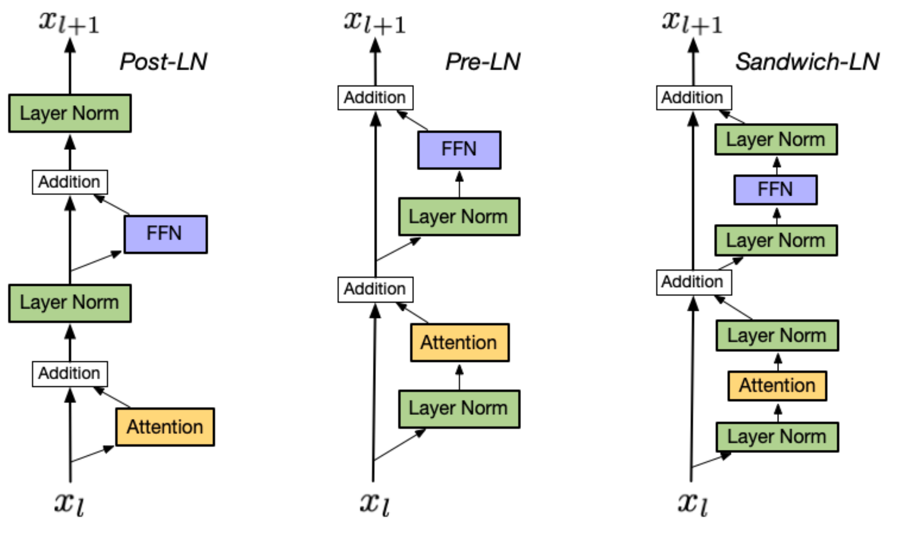
\includegraphics[width=\textwidth]{prepostln}
	\caption{Illustration of different LayerNorm structures in Transformers. Source: \textcite{ding2021cogview}.}
	\label{fig:prepostln}
\end{figure}

The position of the normalization layer (Figure~\ref{fig:prepostln}) in the Transformer architecture can have a significant impact on the model's performance and convergence.
The three main configurations proposed in different studies are pre-LN\footnote{Pre-Layer Normalization}, post-LN\footnote{Post-Layer Normalization}, and Sandwich-LN\@.

In the pre-LN configuration, the normalization layer is placed inside the residual blocks, while in the post-LN configuration, the normalization layer is placed after the residual blocks.
In \textcite{ding2021cogview}, the normalization layer is placed both before and after the residual blocks, which is referred to as the Sandwich-LN configuration.

Post-LN is used in the vanilla Transformer architecture~\cite{vaswani2023attention}, where the normalization layer is placed between the residual blocks.
This sequence allows the model to first process the input through a sublayer, such as a Multi-Head Attention (MHA) or Feed-Forward Network (FFN), and then apply normalization to the output of the sublayer combined with the residual connection.
In particular, to train the model from scratch, any gradient-based optimization approach requires a learning rate warm-up stage to stabilize the training process~\cite{vaswani2023attention}.
Existing works found that training of Transformer models with post-norm tends to be instable due to large gradients near the output layer~\cite{xiong2020layer}.

Pre-LN~\cite{baevski2019adaptive} is another configuration where the normalization layer is placed inside the residual blocks and makes possible to remove warm-up stage, requiring significantly less training time and hyper-parameter tuning on a wide range of applications.
The Transformers with pre-LN have shown to be more stable during training but have worst performance~\cite{liu2020understanding}.

Sandwich-LN~\cite{ding2021cogview} is a configuration that combines the advantages of both pre-LN and post-LN by placing the normalization layer both before and after the residual blocks.
This configuration has been shown to improve the performance of Transformer models by providing better stability during training and faster convergence~\cite{ding2021cogview}.
In \textcite{zeng2022glm130b}, the authors found that the Sandwich-LN configuration sometimes fails to stabilize the training of LLMs and may lead to the collapse of training.

\subsubsection{Activation Functions}
\label{subsubsec:activation-functions}

Activation functions play a crucial role in the training and performance of LLMs by introducing non-linearity into the model\footnote{In the feed-forward layer}.
The most commonly used activation functions in LLMs are ReLU, GeLU, Swish, SwiGLU, and GeGLU\@.

ReLU\footnote{Rectified Linear Unit}~\cite{nair2010rectified} is a simple and widely used activation function that introduces non-linearity by setting negative values to zero.

\begin{equation}
	\text{ReLU}(x) = \max(x, 0)
	\label{eq:relu}
\end{equation}

One of the first activation functions to be used in deep learning, ReLU has been shown to be effective in training deep neural networks by preventing the vanishing gradient problem~\cite{glorot2011deep}.
This non-linear activation function introduces sparsity in the activations of the network, which can lead to faster training and better performance due to its simplicity and efficiency.
However, ReLU can suffer from the dying ReLU problem, where neurons can become inactive and stop learning if the input is negative~\cite{maas2013rectifier}.

GeLU~\cite{hendrycks2016gaussian} is a Gaussian Error Linear Unit (GeLU) activation function that is used to model uncertainties in neural networks.
It was introduced to improve upon ReLU by taking into account the stochastic regularisation techniques.
The GELU activation function is mathematically described as:

\begin{equation}
	\text{GeLU}(x) = x \cdot \Phi(x)
	\label{eq:geluf}
\end{equation}

\noindent where \(\Phi(x)\) is the cumulative distribution function of the standard Gaussian distribution.
This can also be approximated as:

\begin{equation}
	\text{GeLU}(x) \approx 0.5x(1 + \tanh[\sqrt{2/\pi}(x + 0.044715x^3))]
	\label{eq:gelu}
\end{equation}

The GELU function allows the input to control its own gate, deciding whether to pass through or be dampened.
When x is large, GELU approximates to x, acting like a linear unit.
When x is close to zero or negative, it squashes the output, making it closer to zero.
In other words, the GELU function would produce outputs that are smoothed around zero, rather than sharply cut off as with ReLU\@.

The Swish~\cite{ramachandran2017searching} activation function is a smooth, non-monotonic function that was developed to overcome some limitations of ReLU and was found to perform better in deeper models.
It is defined as

\begin{equation}
	\text{Swish}(x) = x \cdotp \sigma(x)
	\label{eq:swish}
\end{equation}

\noindent where x is the input to the activation function and sigmoid is the logistic function \(\sigma(x) = \frac{1}{1+e^{-x}}\).
The Swish function allows small and negative values to pass through, which can be beneficial for gradient flow in deep models.
It has been empirically demonstrated to work well for deeper models and is computationally efficient.

SwiGLU~\cite{shazeer2020glu} is a variant of the Swish activation function that combines the Swish function with the Gated Linear Unit (GLU) function.
The SwiGLU activation function is defined as

\begin{equation}
	\text{SwiGLU}(x_1, x_2) = \text{Swish}(x_1) \odot x_2
	\label{eq:swiglu}
\end{equation}

\noindent where \(x_1\) and \(x_2\) are the input vectors, \(\odot\) denotes element-wise multiplication, and Swish is the Swish activation function described in Equation~\ref{eq:swish}.
This function allows the network to learn which parts of the input should be retained (gated) for further layers, combining the advantages of non-saturating functions and dynamic gating mechanisms.
Note that in practice, \(x_1\) and \(x_2\) often originate from splitting a larger tensor along the feature dimension, and the function is applied across all corresponding elements of the two halves.

GeGLU~\cite{shazeer2020glu} is another variant of the Swish activation function that combines the GeLU function with the GLU function.
The GeGLU activation is formulated as:

\begin{equation}
	\text{GeGLU}(x_1, x_2) = \text{GeLU}(x_1) \odot x_2
	\label{eq:geglu}
\end{equation}

\noindent Here, \(x_1\) and \(x_2\) are the input vectors, \(\odot\) denotes element-wise multiplication, and GeLU is defined in Equation~\ref{eq:geluf}.

\subsubsection{Position Embeddings}
\label{subsubsec:position-embeddings}

Position embeddings are a crucial component of the Transformer architecture that allows the model to capture the sequential order of tokens in the input sequence.
There are several types of position embeddings used in LLMs, including absolute, relative, RoPE, and Alibi embeddings.

Absolute position embeddings~\cite{vaswani2023attention} proposed in the original Transformer model.
At the bottoms of the encoder and the decoder, the absolute positional embeddings are added to the input embeddings.
There are two variants of absolute position embeddings, i.e., sinusoidal and learned position embeddings, where the latter is commonly used in existing pre-trained language models.
The formulation for adding absolute position embeddings is straightforward:

\begin{equation}
	E_{\text{total}}(i) = E_{\text{token}}(i) + E_{\text{position}}(i)
	\label{eq:absolute-position-embeddings}
\end{equation}

\noindent where \(E_{\text{total}}(i)\) is the final embedding vector for token \(i\), \(E_{\text{token}}(i)\) is the initial token embedding for token \(i\), and \(E_{\text{position}}(i)\) is the position embedding vector for token \(i\).
This technique allows the model to use the order of words to understand meaning and context, which is especially important for tasks involving sequence modeling and generation.

Relative position embeddings~\cite{shaw2018self} are an alternative to absolute position embeddings that capture the relative distance between tokens in the input sequence.
This allows the model to learn more flexible and adaptive representations of the input sequence, which can improve performance on tasks that require capturing long-range dependencies and complex relationships between tokens.
Relative position embeddings are incorporated into the self-attention mechanism of Transformer models.
Instead of only considering the absolute position of tokens, the attention scores are adjusted based on the relative distances between tokens.
The formulation for the attention mechanism with relative position embeddings is given by:

\begin{equation}
	\text{Attention}(Q, K, V) = \text{softmax}\left(\frac{Q(K+R)^T}{\sqrt{d_k}}\right)V
	\label{eq:relative-position-embeddings}
\end{equation}

\noindent where \(Q\), \(K\), and \(V\) are the query, key, and value matrices, respectively, \(R\) is the relative position embedding matrix, and \(d_k\) is the dimension of the key vectors.
The relative positions are calculated as \(R_{ij} = R_{pos[i]-pos[j]}\), where \(pos[i]\) and \(pos[j]\) are the positions of tokens \(i\) and \(j\) in the input sequence, respectively.

RoPE\footnote{Rotary Position Embeddings}~\cite{su2021roformer} is a type of position embedding that uses rotational matrices to capture the relative positions of tokens in the input sequence.
Unlike traditional position embeddings that add or concatenate position information, RoPE encodes position information through rotation in the embedding space, enabling models to preserve positional relationships effectively.
The key idea of RoPE is to bind the position encoding with the word embedding in a way that preserves the rotational relationship between embeddings.
It uses a rotation matrix to modulate the embedding based on its position, thereby aligning words by their relative positions instead of their absolute positions.
The formula for the Rotary Position Embedding is:

\begin{equation}
	E_{\text{rot}}(x_i,p_i) = \text{Rotate}(x_i,p_i) = x_i\cos(p_i) + (Wx_i)\sin(p_i)
	\label{eq:rope}
\end{equation}

\noindent where \(x_i\) is the token embedding, \(p_i\) is the position embedding, and \(W\) is a learnable weight matrix.
Rotary Position Embeddings were introduced by \textcite{su2021roformer} and have been shown to improve the performance of LLMs on a range of tasks.

ALiBi\footnote{Attention with Linear Biases}~\cite{press2022train} position embeddings offer an alternative mechanism for incorporating position information into Transformer models.
Unlike traditional absolute or relative position embeddings, ALiBi introduces biases directly into the self-attention mechanism to handle positional dependencies.
ALiBi introduces a linear bias based on the distance between tokens in the attention scores.
This bias is subtracted from the attention logits before the softmax operation, helping the model to prioritize nearby tokens over distant ones, which is crucial in many sequential tasks.
The modified attention score with ALiBi can be represented as:

\begin{equation}
	\begin{aligned}
		\text{Attention}(Q, K, V) & = \text{softmax}\left(\frac{QK^T}{\sqrt{d_k}} - \text{bias}(i,j)\right)V, \\
		\text{bias}(i,j)          & = b \cdotp |i-j|
	\end{aligned}
	\label{eq:alibi}
\end{equation}

\noindent where \(Q\), \(K\), and \(V\) are the query, key, and value matrices, respectively, and \(b\) is a learnable scalar parameter that controls the strength of the bias, and \(|i-j|\) is the absolute distance between tokens \(i\) and \(j\), and \(d_k\) is the dimension of the key vectors.

\subsubsection{Position Attention}
\label{subsubsec:position-attention}
\lipsum[1]


\subsection{Emerging architectures}
\label{subsec:emerging-architectures}

There are several emerging architectures that have been proposed to address specific challenges or improve the performance of the Transformers.
One of the main issues with the vanilla Transformer architecture is the quadratic complexity in terms of the number of tokens, which can limit the model's scalability to longer sequences.
To address this performance issue, several studies proposed alternative architectures, such as parameterized state space models (e.g., S4~\cite{gu2022efficiently}, GSS~\cite{mehta2022long}, and H3~\cite{dao2022hungry}]), long convolutions(e.g.,Hyena~\cite{poli2023hyena}), and recursive update mechanisms (RWKV~\cite{peng2023rwkv} and RetNet~\cite{sun2023retentive}).

